\documentclass[aspectratio=169, table]{beamer}

\usepackage{colortbl}
\usepackage{xcolor}
\usepackage{listings}
\usepackage{tikz}
\usepackage{pgfplots}
\usepgfplotslibrary{polar}
\usetikzlibrary{arrows.meta, positioning, calc}

\usetheme{Pradita}


\usepackage{listings}
\lstdefinestyle{SqlStyle}{
language=SQL,
basicstyle=\ttfamily\footnotesize,
morekeywords={REAL, TEXT, REFERENCES},
keywordstyle=\color{blue},
commentstyle=\color{gray},
stringstyle=\color{red},
breaklines=true,
showstringspaces=false,
tabsize=2,
captionpos=b,
numbers=left,
numberstyle=\tiny\color{gray},
frame=lines,
backgroundcolor=\color{lightgray!10},
comment=[l]{//},
morecomment=[s]{/*}{*/},
commentstyle=\color{gray}\ttfamily,
string=[s]{'}{'},
morestring=[s]{"}{"},
%	stringstyle=\color{teal}\ttfamily,
%	showstringspaces=false
}

\lstdefinelanguage{bash} {
keywords={},
basicstyle=\ttfamily\small,
keywordstyle=\color{blue}\bfseries,
ndkeywords={iex},
ndkeywordstyle=\color{purple}\bfseries,
sensitive=true,
commentstyle=\color{gray},
stringstyle=\color{red},
numbers=left,
numberstyle=\tiny\color{gray},
breaklines=true,
frame=lines,
backgroundcolor=\color{lightgray!10},
tabsize=2,
comment=[l]{\#},
morecomment=[s]{/*}{*/},
commentstyle=\color{gray}\ttfamily,
stringstyle=\color{purple}\ttfamily,
showstringspaces=false
}

% Define Java language style for listings
\lstdefinestyle{JavaScript}{
	language=Java,
	basicstyle=\ttfamily\footnotesize,
	keywordstyle=\color{blue},
	commentstyle=\color{gray},
	stringstyle=\color{red},
	breaklines=true,
	showstringspaces=false,
	tabsize=4,
	captionpos=b,
	numbers=left,
	numberstyle=\tiny\color{gray},
	frame=lines,
	backgroundcolor=\color{lightgray!10},
	comment=[l]{//},
	morecomment=[s]{/*}{*/},
	commentstyle=\color{gray}\ttfamily,
	string=[s]{'}{'},
	morestring=[s]{"}{"},
	%	stringstyle=\color{teal}\ttfamily,
	%	showstringspaces=false
}

\title{\Huge Data Cleaning \\
\vspace{10pt}
and Preparation}
\subtitle{IT140704 - Big Data for Business}
%\date[Serial]{Penggunaan Large Language Model untuk Pengajaran}
\author{\textbf{Alfa Yohannis}}
\begin{document}

\frame{\titlepage}


\begin{frame}[fragile]
\frametitle{Contents}
\vspace{20pt}
\begin{columns}[t]
	\column{0.5\textwidth}
	\tableofcontents[sections={1-4}]
	
	\column{0.5\textwidth}
	\tableofcontents[sections={5-20}]
\end{columns}
\end{frame}

\begin{frame}{\hfill}
	\centering
	\Huge{\textbf{What are the risks and trade-offs of using raw data directly for big data analytics without cleaning and preparation?}}
\end{frame}

\section{Introduction}

\begin{frame}{Introduction}
	\vspace{20pt}
	
	\begin{itemize}
		\item Data cleaning and preparation are fundamental steps in data analysis.
		
		\item High-quality data ensures accurate and reliable analysis and decision-making.
		
		\item Without these processes, advanced analysis and visualisation can be misleading.
		
		\item \textbf{Data cleaning:} identifying and correcting errors, missing values, outliers, or duplicates.
		
		\item \textbf{Data preparation:} transforming, integrating, and organising data for analysis.
		
		\item Business data comes from various sources with different formats and quality.
		
		\item Understanding these processes helps management value the effort before data provides meaningful insights.
		
		\item This chapter introduces key concepts, techniques, and challenges in data cleaning and preparation for effective analysis and strategic business decisions.
	\end{itemize}
	
\end{frame}

\section{Understanding Data Quality}

\begin{frame}{Definition and Importance of Data Quality}
	\vspace{20pt}
	
	\begin{itemize}
		\item \textbf{Definition:} Data quality is how accurate, complete, reliable, and relevant data is.
		
		\item \textbf{Benefits:} High-quality data supports effective decisions, operational efficiency, and strategic planning.
		
		\item \textbf{Risks:} Poor data quality leads to wrong analysis, bad decisions, and financial loss.
		
		\item \textbf{Key dimensions:} accuracy, completeness, consistency, timeliness, validity.
		
		\item \textbf{Accuracy:} correct data; \textbf{Completeness:} all data available; \textbf{Consistency:} same across systems.
		
		\item \textbf{Timeliness:} up-to-date; \textbf{Validity:} meets required formats or rules.
		
		\item \textbf{Importance:} Understanding data quality prevents decisions based on bad data.
	\end{itemize}
	
\end{frame}

\begin{frame}{Data Quality Dimensions}
	\vspace{20pt}
	\centering
	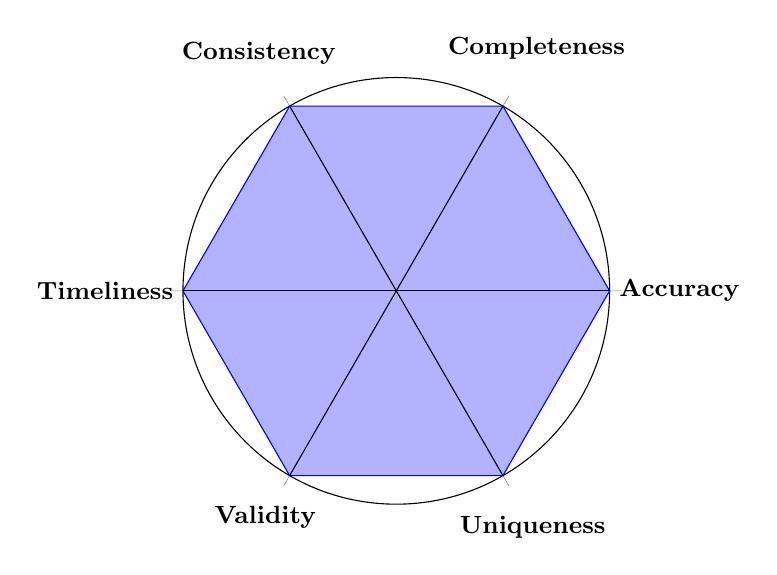
\begin{tikzpicture}[scale=1]
		\begin{polaraxis}[
			width=7cm,
			height=7cm,
			grid=none, % disable default grid to customise lines
			xtick=data,
			xticklabels={\textbf{Accuracy}, \textbf{Completeness}, \textbf{Consistency}, \textbf{Timeliness}, \textbf{Validity}, \textbf{Uniqueness}},
			tick label style={font=\small},
			ylabel=,
			ytick=\empty,
			ymin=0, ymax=1,
			]
			% Draw filled polygon for dimensions
			\addplot[fill=blue!30, draw=blue] coordinates {
				(0,1)
				(60,1)
				(120,1)
				(180,1)
				(240,1)
				(300,1)
				(360,1)
			};
			
			% Add radial lines from center to each dimension
			\draw[black] (axis cs:0,0) -- (axis cs:0,1);
			\draw[black] (axis cs:60,0) -- (axis cs:60,1);
			\draw[black] (axis cs:120,0) -- (axis cs:120,1);
			\draw[black] (axis cs:180,0) -- (axis cs:180,1);
			\draw[black] (axis cs:240,0) -- (axis cs:240,1);
			\draw[black] (axis cs:300,0) -- (axis cs:300,1);
			
		\end{polaraxis}
	\end{tikzpicture}
\end{frame}

\begin{frame}{Data Quality Dimensions}
	\vspace{20pt}
	
	\begin{itemize}
		\item Data quality has dimensions that determine its usability.
		
		\item \textbf{Accuracy}: data correctly represents reality, e.g. customer birthdate is correct.
		
		\item \textbf{Completeness}: all required data is available, e.g. customer income is not missing.
		
		\item \textbf{Consistency}: data is the same across systems, e.g. customer address matches in sales and billing.
		
		\item \textbf{Timeliness}: data is up-to-date and relevant, e.g. current market prices.
		
		\item \textbf{Validity}: data follows required formats or rules, e.g. valid postal codes.
		
		\item \textbf{Uniqueness}: each entity is recorded once without duplication, e.g. customer not counted twice.
	\end{itemize}
	
\end{frame}

\section{Overview of Data Cleaning and Preparation}

\begin{frame}{Definition of Data Cleaning}
	\vspace{20pt}
	
	\begin{itemize}
		\item \textbf{Definition:} Data cleaning identifies and fixes errors, inconsistencies, or inaccuracies to improve data quality.
		
		\item \textbf{Scope:} Handling missing values, removing duplicates, fixing typos, resolving inconsistencies.
		
		\item \textbf{Importance:} Ensures data for planning, monitoring, and customer analysis is reliable.
		
		\item \textbf{Example:} Wrong or inactive emails cause failed marketing campaigns, wasting resources.
		
		\item \textbf{Time:} Takes up to 80\% of analyst or data scientist time.
		
		\item \textbf{Impact:} Prevents costly mistakes like incorrect forecasts or compliance risks.
		
		\item \textbf{Foundation:} Enables meaningful, reliable insights from data preparation and analysis.
	\end{itemize}
	
\end{frame}


\begin{frame}{Definition of Data Preparation}
	\vspace{20pt}
	
	\begin{itemize}
		\item \textbf{Definition:} Data preparation transforms raw data into a form suitable for analysis and decision-making.
		
		\item \textbf{Steps:} Includes cleaning, integration, transformation, reduction, and formatting for analytics or reporting use.
		
		\item \textbf{Business importance:} Enables analysts to convert scattered, inconsistent, or unstructured data into structured datasets that answer business questions.
		
		\item \textbf{Example:} Preparing sales data may merge records from stores, standardise product codes, aggregate weekly sales, and reformat dates consistently.
		
		\item \textbf{Impact:} Effective data preparation improves analytical efficiency and accuracy, supporting decisions, performance monitoring, and strategic planning.
	\end{itemize}
	
\end{frame}

\begin{frame}{Data Preparation Structure and Components}
	\vspace{20pt}
	\centering
	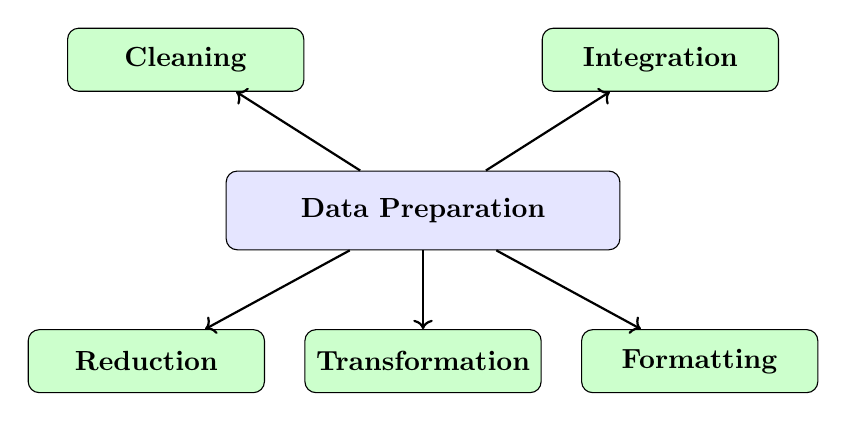
\begin{tikzpicture}[
		node distance=.5cm and .5cm,
		box/.style={rectangle, draw=black, fill=blue!10, rounded corners, minimum width=5cm, minimum height=1cm, align=center},
		subbox/.style={rectangle, draw=black, fill=green!20, rounded corners, minimum width=3cm, minimum height=0.8cm, align=center},
		arrow/.style={->, thick}
		]
		
		% Main Data Preparation box at centre
		\node[box] (prep) {\textbf{Data Preparation}};
		
		% Two components above shifted left and right
		\node[subbox, above left=1cm and -1cm of prep] (clean) {\textbf{Cleaning}};
		\node[subbox, above right=1cm and -1cm of prep] (integration) {\textbf{Integration}};
		
		% Three components below
		\node[subbox, below=1cm of prep] (transform) {\textbf{Transformation}};
		\node[subbox, left=of transform] (reduction) {\textbf{Reduction}};
		\node[subbox, right=of transform] (formatting) {\textbf{Formatting}};
		
		% Inclusion arrows from Preparation to subprocesses
		\draw[arrow] (prep) -- (clean);
		\draw[arrow] (prep) -- (integration);
		\draw[arrow] (prep) -- (transform);
		\draw[arrow] (prep) -- (reduction);
		\draw[arrow] (prep) -- (formatting);
		
	\end{tikzpicture}
\end{frame}



\begin{frame}{Data Cleaning and Preparation}
	\vspace{20pt}
	
	\begin{itemize}
		\item Data cleaning and preparation are related but different concepts.
		
		\item \textbf{Data cleaning} is a sub-process of preparation focused on identifying and fixing errors, inconsistencies, and inaccuracies to ensure data quality.
		
		\item \textbf{Data preparation} is broader, including cleaning plus integration (combining datasets), transformation (changing format or structure), reduction (selecting relevant variables or aggregating), and formatting (ensuring correct input formats).
		
		\item Simply, cleaning ensures data is correct and reliable, while preparation ensures data is ready for its purpose.
		
		\item Both are essential for accurate analysis and successful business decisions.
	\end{itemize}
	
\end{frame}


\begin{frame}{Key Data Cleaning Techniques and Examples}
	\vspace{20pt}
	\centering
	\renewcommand{\arraystretch}{1.2}
	\begin{tabular}{|p{0.3\textwidth}|p{0.6\textwidth}|}
		\hline
		\textbf{Data Cleaning Technique} & \textbf{Implementation Example} \\
		\hline
		Handling Missing Values & Imputing missing customer ages with the average of similar age groups \\
		\hline
		Handling Outliers & Log transformation on extreme income data to reduce influence \\
		\hline
		Data Normalisation & Min-Max scaling sales column to 0–1 scale before analysis \\
		\hline
		Removing Duplicates & Removing duplicate customer entries when merging data from two stores \\
		\hline
		Correcting Data Entry Errors & Correcting typos in product codes or standardising date formats \\
		\hline
	\end{tabular}
\end{frame}

\begin{frame}{Key Data Cleaning Techniques}
	\vspace{20pt}
	
	\begin{itemize}
		\item \textbf{Handling Missing Values:} remove rows with few missing values or impute using mean, median, mode, or predicted values.
		
		\item \textbf{Handling Outliers:} investigate outliers; remove or transform (e.g. log scaling) if needed.
		
		\item \textbf{Data Normalisation:} scale data to common ranges using Min-Max scaling or Z-score standardisation to avoid dominance by large-scale variables.
		
		\item \textbf{Removing Duplicates:} delete duplicate records to ensure each entity is counted once.
		
		\item \textbf{Fixing Input Errors:} correct typos and standardise formats such as dates or product codes.
		
		\item These techniques improve data quality and reliability for accurate business decisions.
	\end{itemize}
	
\end{frame}


\section{Data Integration}

\begin{frame}{Definition and Purpose of Data Integration}
	\vspace{20pt}
	
	\begin{itemize}
		\item \textbf{Definition:} Data integration combines data from multiple sources into a unified, consistent dataset for analysis and decisions.
		
		\item \textbf{Purpose:}
		\begin{itemize}
			\item \textbf{Holistic view:} analyse all relevant data in one place.
			\item \textbf{Better decisions:} managers use complete, consistent information.
			\item \textbf{Operational efficiency:} reduces duplication, streamlines processes, improves communication.
			\item \textbf{Data consistency:} avoids conflicting reports or decisions from incomplete data.
		\end{itemize}
		
		\item \textbf{Example:} Integrating inventory and sales data enables accurate demand forecasting and efficient stock management.
		
		\item Data integration prepares data for analysis, supporting strategic and operational goals.
	\end{itemize}
	
\end{frame}

\begin{frame}{Data Integration Techniques}
	\vspace{20pt}
	\centering
	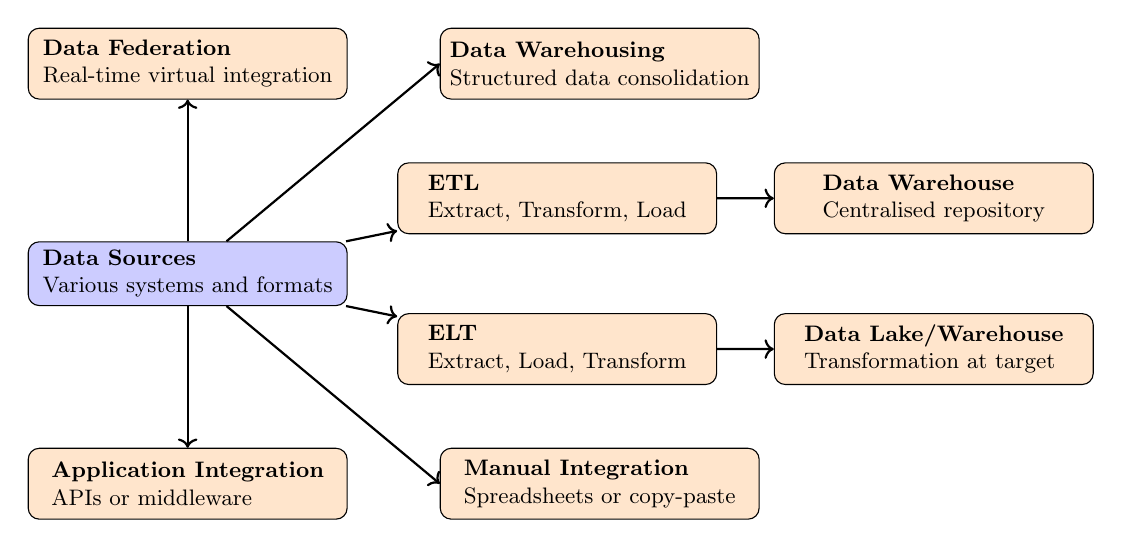
\begin{tikzpicture}[scale=0.9, transform shape, % scale the whole figure
		node distance=0.5cm and 0.8cm,
		box/.style={rectangle, draw=black, fill=orange!20, rounded corners, minimum width=4.5cm, minimum height=1cm, align=left, font=\small},
		sourcebox/.style={rectangle, draw=black, fill=blue!20, rounded corners, minimum width=4.5cm, minimum height=0.5cm, align=left, font=\small},
		arrow/.style={->, thick}
		]
		
		% Source systems node (different color)
		\node[sourcebox] (sources) {\textbf{Data Sources}\\Various systems and formats};
		
		% ETL
		\node[box, above right=.1cm and .7cm of sources] (etl) {\textbf{ETL}\\Extract, Transform, Load};
		\draw[arrow] (sources) -- (etl);
		\node[box, right=of etl] (dw1) {\textbf{Data Warehouse}\\Centralised repository};
		\draw[arrow] (etl) -- (dw1);
		
		% ELT
		\node[box, below right=.1cm and .7cm of sources] (elt) {\textbf{ELT}\\Extract, Load, Transform};
		\draw[arrow] (sources) -- (elt);
		\node[box, right=of elt] (dw2) {\textbf{Data Lake/Warehouse}\\Transformation at target};
		\draw[arrow] (elt) -- (dw2);
		
		% Data Federation
		\node[box, above=2cm of sources] (federation) {\textbf{Data Federation}\\Real-time virtual integration};
		\draw[arrow] (sources) -- (federation);
		
		% Data Warehousing (direct)
		\node[box, right=1.3cm of federation] (warehouse) {\textbf{Data Warehousing}\\Structured data consolidation};
		\draw[arrow] (sources) -- (warehouse.west);
		
		% Application-Based Integration
		\node[box, below=2cm of sources] (appint) {\textbf{Application Integration}\\APIs or middleware};
		\draw[arrow] (sources) -- (appint);
		
		% Manual Integration
		\node[box, right=1.3cm of appint] (manual) {\textbf{Manual Integration}\\Spreadsheets or copy-paste};
		\draw[arrow] (sources) -- (manual.west);
		
	\end{tikzpicture}
\end{frame}

\begin{frame}{Data Integration Techniques}
	\vspace{20pt}
	
	\begin{itemize}
		\item \textbf{ETL (Extract, Transform, Load):} extract from sources, transform to standard format, load to target (e.g. data warehouse).
		
		\item \textbf{ELT (Extract, Load, Transform):} extract and load to target (e.g. data lake), then transform within it.
		
		\item \textbf{Data Federation:} integrates data virtually in real-time without moving it physically.
		
		\item \textbf{Data Warehousing:} centralises cleaned, transformed data for efficient BI queries.
		
		\item \textbf{Application-based Integration:} systems connect directly via APIs (e.g. CRM updates ERP inventory).
		
		\item \textbf{Manual Integration:} using spreadsheets for small-scale, ad-hoc data merges; not scalable.
		
		\item Each technique has strengths depending on structure, scale, and real-time needs.
	\end{itemize}
	
\end{frame}

\begin{frame}{Challenges in Data Integration}
	\vspace{20pt}
	
	\begin{itemize}
		\item \textbf{Data heterogeneity:} differing formats and structures across sources (e.g. date formats).
		
		\item \textbf{Schema and semantic differences:} varied naming or meanings (e.g. “CustomerID” vs “CustNum”; “sales” as gross vs net).
		
		\item \textbf{Data quality issues:} missing values, duplicates, inaccuracies magnified when combined.
		
		\item \textbf{Scalability and performance:} large or real-time integration strains system resources.
		
		\item \textbf{Security and privacy:} moving sensitive data requires compliance and protection.
		
		\item \textbf{Organisational and governance:} aligning departments, ownership, and policies for consistency.
		
		\item Addressing these needs technical solutions, clear policies, and business-IT collaboration for reliable integration.
	\end{itemize}
	
\end{frame}

\section{Maintaining Data Consistency}

\begin{frame}{Definition and Importance of Data Consistency}
	\vspace{20pt}
	
	\begin{itemize}
		\item \textbf{Definition:} Data consistency ensures uniform, coherent data across datasets, systems, and processes.
		
		\item \textbf{Example:} Customer address updated in sales DB but not in delivery system causes shipping errors; differing revenue figures between accounting and sales DB lead to wrong decisions.
		
		\item \textbf{Importance:}
		\begin{itemize}
			\item Better decisions based on reliable, consistent data.
			\item Operational efficiency without delays or errors.
			\item Regulatory compliance avoiding penalties.
			\item Improved customer experience through accurate, personalised communication.
		\end{itemize}
		
		\item Ensuring consistency requires strong data governance, integration, and regular validation across systems.
	\end{itemize}
	
\end{frame}

\begin{frame}{Methods to Maintain Data Consistency}
	\vspace{20pt}
	
	\begin{itemize}
		\item \textbf{Master Data Management (MDM):} create a single authoritative source for key data (e.g. customers, products).
		
		\item \textbf{Data validation rules:} enforce standards during entry or integration (e.g. date formats, valid codes).
		
		\item \textbf{Referential integrity constraints:} ensure database relationships remain valid (e.g. orders link to existing customers).
		
		\item \textbf{Data synchronisation:} updates in one system reflect in others via batch jobs, real-time APIs, or middleware.
		
		\item \textbf{Regular audits and reconciliation:} compare data across systems to detect and fix inconsistencies.
		
		\item \textbf{Clear data governance policies:} define ownership, update responsibilities, and change management procedures.
	\end{itemize}
	
\end{frame}


\begin{frame}{Implications of Inconsistent Data}
	\vspace{20pt}
	
	\begin{itemize}
		\item \textbf{Poor decisions:} conflicting reports lead to wrong budgets, inventory, or market strategies.
		
		\item \textbf{Reduced operational efficiency:} staff spend time reconciling data, slowing processes and raising costs.
		
		\item \textbf{Compliance risks:} inaccurate reports can breach regulations, cause fines, and damage reputation.
		
		\item \textbf{Customer dissatisfaction:} outdated or inconsistent contact data causes failed deliveries and poor service.
		
		\item \textbf{Increased costs:} resolving inconsistencies needs significant resources for cleaning and process redesign.
		
		\item \textbf{Missed opportunities:} unreliable integrated data causes lost market insights or operational improvements.
	\end{itemize}
	
\end{frame}

\section{Case Study}

\begin{frame}{RetailCo System Integration}
	\vspace{20pt}
	\centering
	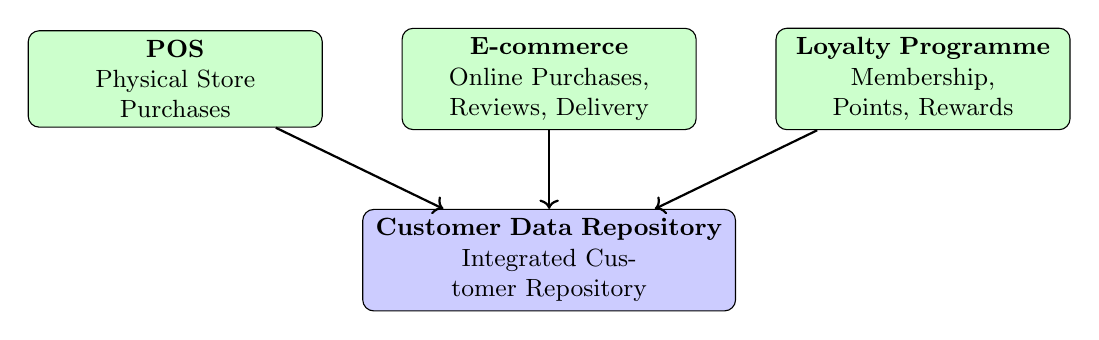
\begin{tikzpicture}[
		scale=1, transform shape, % scale for beamer frame fit
		node distance=1cm and 1cm,
		system/.style={rectangle, draw=black, fill=green!20, rounded corners, text width=3.5cm, minimum height=1cm, align=center, font=\small},
		repo/.style={rectangle, draw=black, fill=blue!20, rounded corners, text width=4.5cm, minimum height=1cm, align=center, font=\small},
		arrow/.style={->, thick}
		]
		
		% Systems
		\node[system] (pos) {\textbf{POS}\\Physical Store Purchases};
		\node[system, right=of pos] (ecom) {\textbf{E-commerce}\\Online Purchases, Reviews, Delivery};
		\node[system, right=of ecom] (loyalty) {\textbf{Loyalty Programme}\\Membership, Points, Rewards};
		
		% Customer Data Repository
		\node[repo, below=1cm of ecom] (cdr) {\textbf{Customer Data Repository}\\Integrated Customer Repository};
		
		% Arrows
		\draw[arrow] (pos) -- (cdr);
		\draw[arrow] (ecom) -- (cdr);
		\draw[arrow] (loyalty) -- (cdr);
		
	\end{tikzpicture}
\end{frame}


\begin{frame}{Overview: Customer Data Integration}
	\vspace{20pt}
	
	\textbf{Case: Customer Data Integration at RetailCo}
	
	RetailCo is a mid-sized retailer with physical stores and an online e-commerce platform. Customer data is stored in separate systems:
	
	\begin{itemize}
		\item POS system: in-store purchase records.
		\item E-commerce platform: online purchases, reviews, shipping details.
		\item Loyalty program: membership info, collected points, redeemed rewards.
	\end{itemize}
	
	Management planned personalised marketing for high-value customers but faced issues:
	
	\begin{itemize}
		\item Names spelled differently (e.g. “John Smith” vs “Jon Smith”).
		\item Birthdates only in e-commerce data.
		\item Outdated or missing emails in loyalty data.
		\item No integrated customer ID across systems.
	\end{itemize}
	
\end{frame}

\begin{frame}{Case Study Analysis: RetailCo}
	\vspace{20pt}
	
	RetailCo’s situation shows common data challenges:
	
	\begin{itemize}
		\item \textbf{Data cleaning:} duplicate customer records with name variations need deduplication and standardisation.
		
		\item \textbf{Data preparation gaps:} no birthdates in POS limits segmentation; solutions include collecting in-store or estimating demographics.
		
		\item \textbf{Integration challenges:} differing customer IDs prevent merging; MDM needed for unified IDs.
		
		\item \textbf{Consistency issues:} outdated or inconsistent emails reduce marketing effectiveness; validation and updates required.
		
		\item \textbf{Business impact:} ineffective targeting, customer dissatisfaction, missed cross-channel revenue opportunities.
	\end{itemize}
	
	Solutions include data cleaning, ETL with MDM integration, and clear data governance policies.
	
\end{frame}


\section{Practical Activity: Evaluating and Preparing Data Without Coding}


\begin{frame}{Online Retail Dataset for Practice}
	\vspace{10pt}
	\url{https://archive.ics.uci.edu/dataset/352/online+retail}
	
	\vspace{10pt}

	\renewcommand{\arraystretch}{1.2}
	\setlength{\arrayrulewidth}{0.3mm} % hairline explicit black border
	\arrayrulecolor{black}
	\centering
		\scriptsize
	\begin{tabular}{|p{0.08\textwidth}|p{0.08\textwidth}|p{0.15\textwidth}|p{0.06\textwidth}|p{0.1\textwidth}|p{0.08\textwidth}|p{0.08\textwidth}|p{0.1\textwidth}|}
		\hline
		\textbf{InvoiceNo} & \textbf{StockCode} & \textbf{Description} & \textbf{Quantity} & \textbf{InvoiceDate} & \textbf{UnitPrice} & \textbf{CustomerID} & \textbf{Country} \\
		\hline
		536365 & 85123A & WHITE HANGING HEART T-LIGHT HOLDER & 6 & 01/12/2010 08:26 & 2.55 & 17850 & United Kingdom \\
		\hline
		536365 & 71053 & WHITE METAL LANTERN & 6 & 01/12/2010 08:26 & 3.39 & 17850 & United Kingdom \\
		\hline
		\multicolumn{8}{c}{\ldots} \\
		\hline
	\end{tabular}
\end{frame}


\begin{frame}{Activity Overview and Dataset}
	\vspace{20pt}
	
	\textbf{Objective:} Practise evaluating, cleaning, preparing, and planning data integration using real datasets with guided tasks and expected solutions.
	
	\textbf{Dataset:}
	\begin{itemize}
		\item \textbf{Online Retail dataset}
		\item Download: \url{https://archive.ics.uci.edu/dataset/352/online+retail}
		\item Open Excel file and review available sheets.
	\end{itemize}
	
	\textbf{Tasks (part 1):}
	\begin{itemize}
		\item \textbf{Identify data quality issues:}
		\begin{itemize}
			\item Missing CustomerID → delete or treat as anonymous.
			\item Inconsistent product descriptions → standardise to title case.
			\item Negative Quantity → classify as returns with indicator column.
		\end{itemize}
	\end{itemize}
	
\end{frame}

\begin{frame}{Activity Tasks (part 2) and Reflection}
	\vspace{20pt}
	
	\textbf{Tasks (part 2):}
	\begin{itemize}
		\item \textbf{Prepare data for analysis:}
		\begin{itemize}
			\item Categorise UnitPrice: <£1 “Low”, £1–£10 “Medium”, >£10 “High”.
			\item Extract month from InvoiceDate for monthly trend analysis.
		\end{itemize}
		
		\item \textbf{Plan data integration:}
		\begin{itemize}
			\item Create a new sheet with CustomerID, AgeGroup, LoyaltyStatus.
			\item Propose left join on CustomerID for segmentation analysis.
		\end{itemize}
		
		\item \textbf{Reflection:}
		\begin{itemize}
			\item Why is data consistency important in sales and customer analysis?
			\item Organisational or technical challenges when integrating transaction and demographic data?
		\end{itemize}
	\end{itemize}
	
	\textbf{Expected Outcome:} Build practical confidence in structured business data preparation without coding.
	
\end{frame}

\section{Summary}

\begin{frame}{Summary}
	\vspace{10pt}
	
	\begin{columns}[T]
		\column{0.5\textwidth}
		\begin{itemize}
			\item Introduced data cleaning and preparation concepts.
			\item Ensuring data is accurate, complete, and analysis-ready.
			\item \textbf{Key cleaning techniques:}
			\begin{itemize}
				\item Handling missing values.
				\item Managing outliers.
				\item Data normalisation.
			\end{itemize}
			\item \textbf{Preparation processes:}
			\begin{itemize}
				\item Data integration.
				\item Maintaining consistency.
			\end{itemize}
		\end{itemize}
		
		\column{0.5\textwidth}
		\begin{itemize}
			\item \textbf{Practical challenges:}
			\begin{itemize}
				\item Organisational – ownership, governance.
				\item Technical – compatibility, scalability.
			\end{itemize}
			\item \textbf{Practical activity:}
			\begin{itemize}
				\item Used Online Retail dataset.
				\item Evaluated data quality.
				\item Planned cleaning steps.
				\item Integrated datasets without coding.
			\end{itemize}
			\item Prepares future managers to lead data-driven projects confidently and collaborate effectively with technical teams.
		\end{itemize}
	\end{columns}
	
\end{frame}

\end{document}
